\documentclass[UTF8,11pt]{ctexart}
\usepackage{graphicx}
\usepackage{amsmath,amsfonts,graphicx,amssymb,bm,amsthm}
\usepackage{enumerate}
\usepackage{color}
\usepackage{geometry} 
\usepackage{listings}
\usepackage{xcolor}
\usepackage[colorlinks,linkcolor=blue]{hyperref} 
\usepackage{amsmath,amsfonts,graphicx,amssymb,bm,amsthm}
\usepackage{listings}
\usepackage{xcolor} % 定制颜色
\definecolor{mygreen}{rgb}{0,0.6,0}
\definecolor{mygray}{rgb}{0.5,0.5,0.5}
\definecolor{mymauve}{rgb}{0.58,0,0.82}
\lstset{ %
backgroundcolor=\color{white},      % choose the background color
columns=flexible,
tabsize=4,
numbers=left,
commentstyle=\color{mygreen},  % comment style
keywordstyle=\color{blue},     % keyword style
stringstyle=\color{mymauve}\ttfamily,  % string literal style
frame=none,
rulesepcolor=\color{red!20!green!20!blue!20},
language = c++,
frame=single
% identifierstyle=\color{red},
}

\hypersetup{colorlinks=true,linkcolor=blue}

\pagestyle{plain}
\geometry{left=2.4cm,right=2.3cm,top=2.0cm,bottom=2.0cm}
\title{rust课程实践报告}
\author{姓名:黄骏齐\and 学号:2100012956} 
\date{2023年7月23日}
\CTEXsetup[format={\Large\bfseries}]{section}
\renewcommand{\refname}{References}

\begin{document}
    \maketitle
    \section*{课程实践报告}
        因为在物理课程上很容易遇到复数的波函数以及积分计算,计划做一个用rust编写的科学计算器,功能包含复数域上的基本运算以及实数域上初等函数的定积分计算。
        
        可以选择使用计算模式还是积分模式。

        \subsection*{复数表达式求值}
            \noindent 实现复数域上的四则运算、指数、对数、三角函数的计算

            \noindent \textbf{输入}:一个合法的表达式,合法的表达式\lstinline|expr|包括:
            \begin{itemize}
                \item 实数\lstinline|a|,纯虚数\lstinline|bi|
                \item 常数\lstinline|e|,\lstinline|pi|
                \item \lstinline|(expr)|,小括号
                \item \lstinline|+expr|,\lstinline|-expr|,单元运算
                \item \lstinline|expr1 op expr2|,二元运算,其中$op \in \{+,-,*,/\}$
                \item \lstinline|expr1^expr2|,要求expr1的值是正实数
                \item \lstinline|ln(expr)|,要求expr的值是正实数
                \item \lstinline|sin(expr),cos(expr),tan(expr)|
            \end{itemize}
            
            运算的优先级是单元运算$>\wedge >*/>+-$,运算法则满足\ref{lalala}

            \noindent 注:表达式可以在不影响意义的情况下任意加空格。还有判断除零、$\tan(\frac{\pi}{2})$等,对数只实现$\ln$,其余需要手动进行换底公式的变换

            \noindent \textbf{输出}:会检测输入的表达式是否合法,若合法,则输出表达式的值(数值表示),否则输出相应的错误信息。
        \subsection*{定积分计算}    
            \noindent \textbf{输入}:\lstinline|a b f(x)|

            \noindent 要求满足$a,b \in \mathbf{R}$,且$f(x)$中只有变元$x$且需要在实数域下,其余的形式满足上面的规则。

            \noindent \textbf{输出}:会检测输入是否合法,若合法,则输出$\int_{a}^{b}f(x)dx$,否则输出相应的错误信息。但不判断被积函数是否一定有意义且可积,如果给了一个合法的输入但是错误的函数,可能会得到错误的结果。

        
        \subsection*{实现方法}

            首先使用了peg Parser\cite{peg}生成器对输入数据进行了一些处理,把一个表达式写成一个enum的形式,enum如下所示:
\begin{lstlisting}
pub enum Node {
    Ident(Complex),
    Dop(char, Box<Node>, Box<Node>),
    Sop(char, Box<Node>)
}
\end{lstlisting}

其中第一行表示单个复数,第二行表示一个二元运算,第三行表示单元运算

然后通过对\lstinline|impl|在\lstinline|Node|上的函数calc进行递归计算值。

在每一层递归中用pattern matching来计算,calc函数如下
\begin{lstlisting}
pub fn calc(self) -> Complex{
    match self{
        Self::Ident(v) => v,
        Self::Dop(c, x,y) => Complex::bopcalc(c,x.calc(),y.calc()),
        Self::Sop(c,x) => Complex::sopcalc(c,x.calc())
    }
}    
\end{lstlisting}

其中|Complex|是一个定义复数的\lstinline|struct|,而\lstinline|bopcalc|和\lstinline|sopcalc|分别是作用在的\lstinline|Complex|上的二元和单元函数。

对于其中的除法、ln、exp运算,则通过使用result类型来判断与记录错误信息

\begin{figure}[!htb]
    \centering
    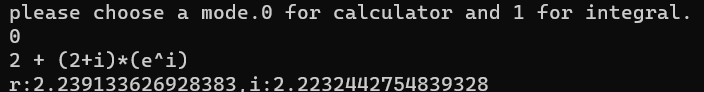
\includegraphics[scale=1.1]{1.png}
    \caption{复数计算器效果}
\end{figure}

对于定积分计算,使用辛普森积分法\ref{hahaha},本质上转化成函数的多点求值问题,多次调用表达式求值,来获得定积分的近似解。

\begin{figure}[!htb]
    \centering
    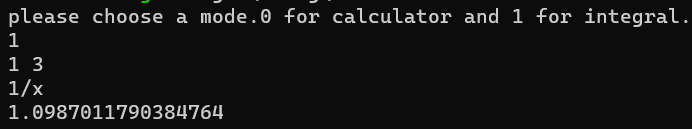
\includegraphics[scale=1.1]{2.png}
    \caption{积分计算器效果,$\ln 3 = 1.09861229$,对数值积分还是有些误差}
\end{figure}

项目地址:\url{https://github.com/huangjunqi1/rustcalculator/}

\section*{todo list}

\begin{itemize}
    \item  一个ui界面
    \item 更好地记录下错误信息
    \item 支持更多函数
    \item 支持读入的科学计数法
    \item 保存之前的结果
\end{itemize}

\section*{附录}
    \subsection{复数域上的运算法则}\label{lalala}
    \begin{itemize}
        \item $i*i = -1$
        \item $(a+bi)*(c+di) = (ac-bd) + (ad+bc)i$
        \item $e^{\theta i} = \cos\theta + i\sin \theta $\cite{Euler}
        \item $\cos x = \frac{e^{ix}+e^{-ix}}{2},\sin x = \frac{e^{ix}-e^{-ix}}{2}$,即复数的三角函数也是有意义的
        \item $\log_a b = \frac{\ln b}{\ln a}$,换底公式
    \end{itemize}
    \subsection{辛普森积分法}\label{hahaha}
        在被积区间中采样$n$个点来得到积分的估计\cite{Simpson},下式中$n$是偶数

        \noindent $\int_{a}^{b}f(x)dx \approx \frac{b-a}{3n}[f(a)+f(b)+4\sum_{i=1}^{n/2}f(x_{2i-1})+2\sum_{i=1}^{n/2-1}f(x_{2i})]$,其中$\{x_i\}$是$[a,b]$的$n$分点

        \noindent 误差为$Err \leq \frac{M(b-a)^5}{180n^4}$,其中$M$是区间上四阶导的最大值

        实际使用20000个分点来求积分的近似值,根据实际运行情况进行调整,在分点上表达式无意义的话则输出错误信息,但不检测其他点上函数是否有值。
\begin{thebibliography}{80}
    \bibitem{peg} \href{https://github.com/kevinmehall/rust-peg}{rust-peg}
    \bibitem{Euler} \href{https://en.wikipedia.org/wiki/Euler%27s_formula}{Euler's formula}
    \bibitem{Simpson} \href{https://en.wikipedia.org/wiki/Simpson%27s_rule}{Simpson's rule}
    \bibitem{fltk} \href{https://github.com/fltk-rs/fltk-rs}{fltk-rs}
\end{thebibliography}


\end{document}

